\section{单纯复形与单纯映射}
\sourcepage{8--9}
\entry{定义}{1.3.1}$\R^N$ 中的\textbf{单纯复形}（simplicial complex）$K$ 是 $\R^N$ 中的一族单形，满足：
\begin{enumerate}[label=(\arabic*)]
\item $K$ 中每个单形的每个面都属于 $K$。
\item $K$ 中任意两个单形的交都是它们各自的一个面。
\end{enumerate}
\entry{例}{1.3.2}图 1.3.1 中的一族单形 $K_1$ 由一个 $2$ 维单形及其各个面组成，是一个单纯复形。$K_2$ 由具有一条公共边的两个 $2$ 维单形及其各个面组成，也是单纯复形；$K_3$ 则不是。那么 $K_4$ 呢？
\begin{center}
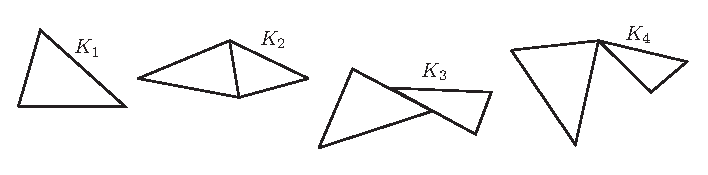
\includegraphics[width=115mm]{figures/1-3-1.pdf}\\图 1.3.1
\end{center}
验证一族单形是否构成单纯复形时，下面的引理有时很有用。

\entry{引理}{1.3.3}一族单形 $K$ 构成单纯复形，当且仅当下列条件成立：
\begin{enumerate}[label=(\arabic*)]
\item $K$ 中每个单形的每个面都属于 $K$。
\item[$(2')$] $K$ 中每一对不同单形的内部不相交。
\end{enumerate}
\noindent\textbf{证明：}先设 $K$ 是单纯复形。给定 $K$ 中两个单形 $\sigma,\tau$，证明：若存在 $x\in\Int\sigma\cap\Int\tau$，则 $\sigma=\tau$。令 $s=\sigma\cap\tau$。如果 $s$ 是 $\sigma$ 的真面，那么 $x$ 就属于 $\Bd\sigma$，这不可能。因此 $s=\sigma$。类似地，$s$ 也不是 $\tau$ 的真面，故 $s=\tau$。由此得到 $\sigma=s=\tau$。

反过来，设 (1) 与 $(2')$ 成立。给定 $K$ 中两个单形 $\sigma,\tau$，假定 $\sigma\cap\tau$ 非空。证明 $\sigma\cap\tau$ 是 $\sigma$ 的一个面 $\sigma'$。具体地，$\sigma'$ 是由 $\sigma$ 的那些属于 $\tau$ 的顶点 $b_0,b_1,\ldots,b_m$ 张成的面。首先，$\sigma'$ 包含在 $\sigma\cap\tau$ 中，因为 $\sigma\cap\tau$ 是包含这些顶点的凸集。为证明反向包含关系，设 $x\in\sigma\cap\tau$。对于 $\sigma$ 的某个面 $s$ 和 $\tau$ 的某个面 $t$，有 $x\in\Int s\cap\Int t$。由 $(2')$ 得 $s=t$。因此 $s$ 的顶点都属于 $\tau$，按定义，它们都属于集合 $\{b_0,\ldots,b_m\}$。所以 $s$ 是 $\sigma'$ 的面，从而得到所需的包含关系。类似地，可以证明 $\sigma\cap\tau$ 是 $\tau$ 的一个面 $\tau'$。这就证明了条件 (2)。\hfill$\square$

由此引理可知，若 $\sigma$ 是单形，则由 $\sigma$ 及其所有真面组成的族是单纯复形：条件 (1) 显然成立；条件 $(2')$ 成立，是因为对于每个点 $x\in\sigma$，恰好存在 $\sigma$ 的一个面 $s$ 使 $x\in\Int s$。

\entry{定义}{1.3.4}若 $L$ 是 $K$ 的一个子族，且包含其各个元素的所有面，则 $L$ 本身也是单纯复形，称为 $K$ 的\textbf{子复形}（subcomplex）。$K$ 的一个子复形是由 $K$ 中维数至多为 $p$ 的所有单形组成的族，称为 $K$ 的 \textbf{$p$ 维骨架}（$p$-skeleton），记作 $K^{(p)}$。族 $K^{(0)}$ 中的点称为 $K$ 的顶点。

\entry{定义}{1.3.5}设 $|K|$ 是 $K$ 的所有单形的并，视为 $\R^N$ 的子集。赋予每个单形作为 $\R^N$ 子空间的自然拓扑，然后如下赋予 $|K|$ 拓扑：规定 $|K|$ 的子集 $A$ 为闭集，当且仅当对每个 $\sigma\in K$，$A\cap\sigma$ 在 $\sigma$ 中是闭集。容易看出这确实定义了一个拓扑，因为这样的集合族对有限并与任意交封闭。空间 $|K|$ 称为 $K$ 的\textbf{底空间}（underlying space），或 $K$ 的\textbf{多胞体}（polytope）。

\sourcepage{10}
作为某个单纯复形的多胞体的空间称为\textbf{多面体}。［注意，有些拓扑学家只把有限单纯复形的多胞体称为多面体。］

一般地，$|K|$ 的这个拓扑比它作为 $\R^N$ 子空间继承的拓扑更细，也就是更大。为说明这一点，注意：若 $A$ 在子空间拓扑下是 $|K|$ 的闭集，则对于 $\R^N$ 的某个闭集 $B$，有 $A=B\cap|K|$。对于 $K$ 中每个单形 $\sigma$，$B\cap\sigma$ 在 $\sigma$ 中闭，因而
\[
A\cap\sigma=B\cap|K|\cap\sigma=B\cap\sigma
\]
在 $\sigma$ 中闭。根据定义，$A$ 在 $|K|$ 的上述拓扑中闭。

一般情况下，$|K|$ 上的子空间拓扑与定义 1.3.5 的拓扑并不相同，见例 1.3.6 和例 1.3.7。不过，若 $K$ 有限，两者就相同。事实上，设 $K$ 有限，且 $A$ 在 $|K|$ 中闭。那么 $A\cap\sigma$ 在 $\sigma$ 中闭，因而在 $\R^N$ 中也闭。由于 $A$ 是有限多个闭集 $A\cap\sigma$ 的并，$A$ 在 $\R^N$ 中也闭。

\entry{例}{1.3.6}设 $K$ 由下列单形及其所有面组成：$\R$ 中所有形如 $[m,m+1]$ 的 $1$ 维单形，其中 $m$ 是非零整数；以及所有形如 $[1/(n+1),1/n]$ 的单形，其中 $n$ 是正整数。那么 $K$ 是一个复形，其底空间作为集合等于 $\R$，但作为拓扑空间则不同。例如，由各点 $1/n$（$n>0$）组成的集合在 $|K|$ 中闭，在 $\R$ 中却不闭。

\entry{例}{1.3.7}设 $K$ 是由 $1$ 维单形 $\sigma_1,\sigma_2,\ldots$ 及其顶点组成的族，其中 $\sigma_i$ 是 $\R^2$ 中以 $0$ 和 $(1,1/i)$ 为顶点的 $1$ 维单形，见图 1.3.2。那么 $K$ 是单纯复形。$|K|$ 与开抛物线弧 $\{(x,x^2):x>0\}$ 的交在 $|K|$ 中是闭集，因为它与每个单形 $\sigma_i$ 的交是单点集。但在 $|K|$ 从 $\R^2$ 继承的拓扑中，它不是闭集，因为在那个拓扑下，原点是它的极限点。
\begin{center}
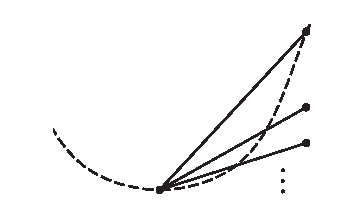
\includegraphics[width=60mm]{figures/1-3-2.pdf}\\图 1.3.2
\end{center}
下面证明多面体的一些初等拓扑性质。

\entry{引理}{1.3.8}若 $L$ 是 $K$ 的子复形，则 $|L|$ 是 $|K|$ 的闭子空间。特别地，若 $\sigma\in K$，则 $\sigma$ 是 $|K|$ 的闭子空间。

\noindent\textbf{证明：}设 $A$ 在 $|L|$ 中闭。若 $\sigma$ 是 $K$ 的一个单形，则 $\sigma\cap|L|$ 是 $\sigma$ 的那些属于 $L$ 的面 $s_i$ 的并。因为 $A$ 在 $|L|$ 中闭，集合 $A\cap s_i$ 在 $s_i$ 中闭，因而在 $\sigma$ 中也闭。由于 $A\cap\sigma$ 是有限多个集合 $A\cap s_i$ 的并，它在 $\sigma$ 中闭。因此 $A$ 在 $|K|$ 中闭。

反过来，若 $B$ 在 $|K|$ 中闭，则对每个 $\sigma\in K$，$B\cap\sigma$ 在 $\sigma$ 中闭，特别是对每个 $\sigma\in L$ 都如此。所以 $B\cap|L|$ 在 $|L|$ 中闭。\hfill$\square$

\sourcepage{11--12}
\entry{引理}{1.3.9}映射 $f:|K|\to X$ 连续，当且仅当对每个 $\sigma\in K$，限制映射 $f|_\sigma$ 连续。

\noindent\textbf{证明：}若 $f$ 连续，则 $f|_\sigma$ 也连续，因为 $\sigma$ 是 $|K|$ 的子空间。反过来，设每个 $f|_\sigma$ 都连续。若 $C$ 是 $X$ 中的闭集，则
\[
f^{-1}(C)\cap\sigma=(f|_\sigma)^{-1}(C),
\]
由 $f|_\sigma$ 的连续性知，这个集合在 $\sigma$ 中闭。因此按定义，$f^{-1}(C)$ 在 $|K|$ 中闭。\translatornote{原文左端印作 $f^{-1}(C\cap\sigma)$；$C$ 与 $\sigma$ 位于不同空间，据上下文应为此处所列等式。}\hfill$\square$

\entry{定义}{1.3.10}设 $X$ 是空间，$\mathcal C$ 是 $X$ 的一族子空间，且其并为 $X$。若 $A$ 在 $X$ 中闭，当且仅当对每个 $C\in\mathcal C$，$A\cap C$ 在 $C$ 中闭，则称 $X$ 的拓扑与族 $\mathcal C$ \textbf{相干}（coherent）。等价地，也可要求：$U$ 在 $X$ 中开，当且仅当对每个 $C\in\mathcal C$，$U\cap C$ 在 $C$ 中开。

特别地，$|K|$ 的拓扑与子空间族 $\{\sigma:\sigma\in K\}$ 相干。

引理 1.3.9 的类似结论对一般的相干拓扑也成立：映射 $f:X\to Y$ 连续，当且仅当对每个 $C\in\mathcal C$，$f|_C$ 连续。

下面把定义 1.2.1 中的重心坐标扩张为定义在多面体上的一族函数。

\entry{定义}{1.3.11}设 $v$ 是单纯复形 $K$ 的任意顶点。如下定义\textbf{重心坐标} $t_v:|K|\to[0,1]$。点 $x\in|K|$ 恰好位于 $K$ 的一个单形的内部，设该单形的顶点为 $a_0,\ldots,a_n$。于是存在正数 $t_0,\ldots,t_n$，使得
\[
x=\sum_{i=0}^n t_i a_i,\qquad \sum_{i=0}^n t_i=1.
\]
若 $v$ 不是其中任何一个顶点 $a_i$，令 $t_v(x)=0$。若 $v$ 是某个顶点，例如 $v=a_{i'}$，则令 $t_v(x)=t_{i'}$。

固定 $v$ 后，函数 $t_v(x)$ 在 $K$ 的每个固定单形 $\sigma$ 上的限制都是连续的，因为它或者在 $\sigma$ 上恒为零，或者等于先前定义的、$x$ 关于 $\sigma$ 的顶点 $v$ 的重心坐标。因此由引理 1.3.9，$t_v(x)$ 在 $|K|$ 上连续。

\entry{引理}{1.3.12}多面体 $|K|$ 是 Hausdorff 空间。

\noindent\textbf{证明：}给定 $|K|$ 中两点 $x_0\ne x_1$，至少存在一个顶点 $v$，使 $t_v(x_0)\ne t_v(x_1)$。在这两个数之间选取 $r$。则集合 $\{x:t_v(x)<r\}$ 与 $\{x:t_v(x)>r\}$ 就是所需的两个不相交开集，分别包含这两个点。\hfill$\square$

\entry{引理}{1.3.13}若 $K$ 有限，则 $|K|$ 紧致。反过来，若 $|K|$ 的子集 $A$ 紧致，则存在 $K$ 的某个有限子复形 $K_0$，使 $A\subset|K_0|$。

\noindent\textbf{证明：}若 $K$ 有限，则 $|K|$ 是有限多个紧致子空间 $\sigma$ 的并，因而紧致。

现设 $A\subset|K|$ 紧致，而且 $A$ 不包含在 $K$ 的任何有限子复形的多胞体中。只要 $A\cap\Int s$ 非空，就从中选取一点 $x_s$。那么集合 $B=\{x_s\}$ 是无限集。此外，$B$ 的每个子集都是闭集，因为它与任何单形 $\sigma$ 的交都是有限集。由于 $B$ 闭且离散，它没有极限点，这与紧致空间的每个无限子集都有极限点这一事实矛盾。\hfill$\square$

研究 $|K|$ 的局部性质时，有三个特定子空间经常有用，现介绍如下。

\entry{定义}{1.3.14}若 $v$ 是 $K$ 的一个顶点，则 $v$ 在 $K$ 中的\textbf{星形邻域}（star），记作 $\operatorname{St}v$，有时也记作 $\operatorname{St}(v,K)$，是 $K$ 中所有以 $v$ 为顶点的单形的内部的并。其闭包记作 $\overline{\operatorname{St}v}$，称为 $v$ 在 $K$ 中的\textbf{闭星形邻域}（closed star）。它是 $K$ 中所有以 $v$ 为顶点的单形的并，也是 $K$ 的某个子复形的多胞体。集合 $\overline{\operatorname{St}v}\setminus\operatorname{St}v$ 称为 $v$ 在 $K$ 中的\textbf{链环}（link），记作 $\operatorname{Lk}v$，见图 1.3.3。
\begin{center}
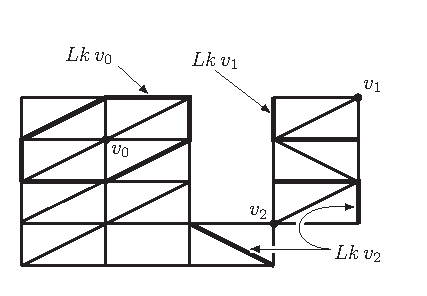
\includegraphics[width=76mm]{figures/1-3-3.pdf}\\图 1.3.3
\end{center}
$\operatorname{St}v$ 在 $|K|$ 中开，因为它恰由满足 $t_v(x)>0$ 的点组成。它的补集是 $K$ 中所有不以 $v$ 为顶点的单形的并，因此是 $K$ 的一个子复形的多胞体。$\operatorname{Lk}v$ 也是 $K$ 的一个子复形的多胞体；它是 $\overline{\operatorname{St}v}$ 与 $\operatorname{St}v$ 的补集的交。容易看出，$\operatorname{St}v$ 和 $\overline{\operatorname{St}v}$ 都道路连通，但 $\operatorname{Lk}v$ 不一定连通。

\sourcepage{13--14}
\entry{定义}{1.3.15}若 $K$ 的每个顶点只属于 $K$ 中有限多个单形，则称单纯复形 $K$ \textbf{局部有限}（locally finite）。换言之，$K$ 局部有限，当且仅当每个闭星形邻域 $\overline{\operatorname{St}v}$ 都是 $K$ 的某个有限子复形的多胞体。

\entry{引理}{1.3.16}复形 $K$ 局部有限，当且仅当空间 $|K|$ 局部紧致。

\noindent\textbf{证明：}设 $K$ 局部有限。给定 $x\in|K|$，它位于 $K$ 的某个顶点 $v$ 的星形邻域 $\operatorname{St}v$ 中。因为 $\overline{\operatorname{St}v}$ 是紧致集，$|K|$ 局部紧致。逆命题留作习题。\hfill$\square$

\subsection*{单纯映射}
现在介绍从一个复形到另一个复形的“单纯映射”的概念。

\entry{引理}{1.3.17}设 $K,L$ 为复形，$f:K^{(0)}\to L^{(0)}$ 为映射。假设只要 $K$ 的顶点 $v_0,v_1,\ldots,v_n$ 张成 $K$ 的一个单形，点 $f(v_0),f(v_1),\ldots,f(v_n)$ 就是 $L$ 的某个单形的顶点。则 $f$ 可以扩张为连续映射 $g:|K|\to|L|$，满足
\[
x=\sum_{i=0}^n t_i v_i\quad\Longrightarrow\quad
g(x)=\sum_{i=0}^n t_i f(v_i).
\]
称 $g$ 为顶点映射 $f$ 诱导的［线性］\textbf{单纯映射}（simplicial map）。

\noindent\textbf{证明：}注意，$L$ 的顶点 $f(v_0),\ldots,f(v_n)$ 虽然不一定互异，但根据假设，它们仍张成 $L$ 的一个单形 $\tau$。把 $g(x)$ 的表达式“合并同类项”之后，系数仍然非负，而且其和仍为 $1$。为说明合并同类项的含义，设 $f(v_0)=f(v_1)$，其余各点 $f(v_2),\ldots,f(v_n)$ 互异。则
\[
g(x)=\sum_{i=0}^n t_i f(v_i)
=(t_0+t_1)f(v_1)+\sum_{i=2}^n t_i f(v_i).
\]
\translatornote{原文末项求和的下限印作 $3$，但紧接着给出的重心坐标包含 $t_2$；这里按合并同类项的含义取 $2$。}
因此，$\tau$ 由 $f(v_1),f(v_2),\ldots,f(v_n)$ 张成，而 $g(x)$ 是 $\tau$ 中重心坐标为 $(t_0+t_1),t_2,\ldots,t_n$ 的点。所以 $g$ 把 $v_0,\ldots,v_n$ 张成的 $n$ 维单形 $\sigma$ 连续地映到顶点集为 $\{f(v_0),\ldots,f(v_n)\}$ 的单形 $\tau$ 中。

$g$ 作为从 $\sigma$ 到 $\tau$ 的映射是连续的，因而作为从 $\sigma$ 到 $|L|$ 的映射也连续。由引理 1.3.9，$g$ 作为从 $|K|$ 到 $|L|$ 的映射连续。\hfill$\square$

从 $K^{(0)}$ 到 $L^{(0)}$ 的顶点映射 $f$ 决定了从 $|K|$ 到 $|L|$ 的扩张 $g$。当然，将 $g$ 限制在顶点集 $K^{(0)}$ 上，就回到原来的映射 $f$。在不致混淆时，有时只用 $g$，或只用 $f$，同时表示这两个映射。

注意，只要 $v_0,v_1,\ldots,v_n$ 张成 $K$ 的一个单形，即使这些点并不互异，$g$ 的公式仍然成立。关键条件是 $t_i$ 非负且其和为 $1$。再一次合并同类项即可看出这一点。

单纯映射 $g:|K|\to|L|$ 与 $h:|L|\to|M|$ 的复合仍为单纯映射。理由如下：设 $\sigma$ 是由 $v_0,\ldots,v_n$ 张成的 $K$ 的单形。根据假设，无论顶点 $g(v_0),\ldots,g(v_n)$ 是否互异，它们都张成 $L$ 的一个单形。同样，无论 $h(g(v_0)),\ldots,h(g(v_n))$ 是否互异，它们也张成 $M$ 的一个单形。对于 $x\in\sigma$，写作 $x=\sum t_i v_i$，其中 $t_i\geq0$、$\sum t_i=1$，利用 $g$ 的公式得
\[
h(g(x))=h\left(\sum_{i=0}^n t_i g(v_i)\right)
=\sum_{i=0}^n t_i h(g(v_i)).
\]
\entry{引理}{1.3.18}设 $f:K^{(0)}\to L^{(0)}$ 是双射，并且 $K$ 的顶点 $v_0,\ldots,v_n$ 张成 $K$ 的一个单形，当且仅当 $f(v_0),\ldots,f(v_n)$ 张成 $L$ 的一个单形。则诱导的单纯映射 $g:|K|\to|L|$ 是同胚。

映射 $g$ 称为 $K$ 到 $L$ 的\textbf{单纯同胚}（simplicial homeomorphism），或\textbf{同构}（isomorphism）。

\noindent\textbf{证明：}$K$ 的每个单形 $\sigma$ 都被 $g$ 映到与它同维的某个单形 $\tau$ 上。只需证明由顶点对应 $f^{-1}$ 诱导的线性映射 $h:\tau\to\sigma$ 是 $g:\sigma\to\tau$ 的逆映射。若 $x=\sum t_i v_i$，则根据定义，$g(x)=\sum t_i f(v_i)$，因此
\[
h[g(x)]=h\left[\sum t_i f(v_i)\right]
=\sum t_i f^{-1}[f(v_i)]=\sum t_i v_i=x.
\]\hfill$\square$

\entry{推论}{1.3.19}以 $\Delta^N$ 表示由一个 $N$ 维单形及其各个面组成的复形。若 $K$ 是有限复形，则对于某个 $N$，$K$ 同构于 $\Delta^N$ 的一个子复形。

\noindent\textbf{证明：}设 $K$ 的顶点为 $v_0,v_1,\ldots,v_N$。在 $\R^N$ 中选取几何独立的点 $a_0,a_1,\ldots,a_N$，令 $\Delta^N$ 由它们张成的 $N$ 维单形及其所有面组成。顶点映射 $f(v_i)=a_i$ 诱导了 $K$ 与 $\Delta^N$ 的某个子复形之间的同构。\hfill$\square$

\subsection*{一般的单纯复形}
要求单纯复形 $K$ 必须位于某个 $\R^N$ 中，会限制 $K$ 的基数和其中单形的维数。现在去掉这些限制。

\sourcepage{15--16}
设 $J$ 为任意指标集，用 $\R^J$ 表示 $\R$ 与自身的 $J$ 重笛卡尔积。$\R^J$ 的元素是从 $J$ 到 $\R$ 的函数，通常用“元组记号”$(x_\alpha)_{\alpha\in J}$ 表示。逐坐标定义通常的加法与标量乘法，乘积 $\R^J$ 自然成为向量空间。

令 $E^J$ 为 $\R^J$ 的如下子集：其中每个点 $(x_\alpha)_{\alpha\in J}$ 除有限多个坐标外，其余坐标都为零。注意，$E^J$ 是 $\R^J$ 的向量子空间。\translatornote{原文此处将环境向量空间写作 $(x_\alpha)_{\alpha\in J}$，据上下文应指 $\R^J$。}设 $\epsilon_\alpha\in E^J$ 是在指标 $\alpha$ 处取值 $1$、在 $J$ 的其他元素处取值 $0$ 的函数，则 $\{\epsilon_\alpha:\alpha\in J\}$ 是 $E^J$ 的一组基；当 $J$ 无限时，它不是 $\R^J$ 的基。

我们称 $E^J$ 为\textbf{广义欧氏空间}（generalized euclidean space），并赋予由度量
\[
|x-y|=\max_{\alpha\in J}|x_\alpha-y_\alpha|
\]
确定的拓扑。

对于 $\R^N$ 中的复形，前面所作的一切都可推广到 $E^J$ 中的复形。空间 $E^J$ 是某些有限维子空间的并，即由基 $\{\epsilon_\alpha:\alpha\in J\}$ 的有限子集张成的各子空间的并。这样的每个子空间都只是某个 $\R^N$ 的副本。$E^J$ 中任意有限点集 $\{a_0,\ldots,a_n\}$ 都位于这样的一个子空间中；若这些点几何独立，则它们张成的单形也位于同一个子空间中。此外，$E^J$ 的度量在每个这样的子空间上给出通常的拓扑。因此，$E^J$ 中任意有限族单形都位于某个 $\R^N$ 的副本中。我们实际所做的，只是允许处理这样的复形：其中所有单形无法整体放入任何一个 $\R^N$ 中。从概念上看，在 $E^J$ 中工作似乎比在 $\R^N$ 中更复杂，但实际上并不造成困难。

请读者验证，我们的结论对于 $E^J$ 中的复形仍然成立。今后我们将自由使用这些结论。

再补充一点：若 $K$ 是 $\R^N$ 中的复形，则其中每个单形的维数至多为 $N$。另一方面，若 $K$ 是 $E^J$ 中的复形，则其中单形的维数不一定有上界。如果 $K$ 中单形的维数存在最大值，就定义此最大值为 $K$ 的\textbf{维数}，记作 $\dim K$；否则，称 $K$ 为无限维的。

\subsection*{习题}
\begin{enumerate}
\item 设 $K$ 为单纯复形，$\sigma\in K$。什么条件下 $\Int\sigma$ 在 $|K|$ 中开？什么条件下 $\sigma$ 在 $|K|$ 中开？
\item 证明，一般地，$\operatorname{St}v$ 和 $\overline{\operatorname{St}v}$ 都道路连通。
\item \begin{enumerate}[label=(\alph*)]
\item 直接证明例 1.3.7 中的多面体不是局部紧致的。
\item 一般地，证明若复形 $K$ 不局部有限，则空间 $|K|$ 不局部紧致。
\end{enumerate}
\item 证明例 1.3.7 中的多面体不可度量化。［提示：证明它不满足第一可数公理。］
\item 若 $g:|K|\to|L|$ 是把 $\sigma$ 的顶点映到 $\tau$ 的顶点上的单纯映射，证明 $g$ 将 $\sigma$ 的某个面同胚地映到 $\tau$ 上。
\item 验证：只要把本节所有八个引理证明中的 $\R^N$ 都换为 $E^J$，这些证明就可原封不动地用于 $E^J$ 中的复形。
\item 设 $K$ 为复形。证明 $|K|$ 可度量化，当且仅当 $K$ 局部有限。［提示：函数 $d(x,y)=\sup_v|t_v(x)-t_v(y)|$ 在 $K$ 的每个有限子复形上都是与其拓扑相容的度量。］
\item 设 $K$ 为复形。证明 $|K|$ 是正规空间。［提示：若 $A$ 在 $|K|$ 中闭，且 $f:A\to[0,1]$ 连续，利用 Tietze 扩张定理，逐步将 $f$ 扩张到 $A\cup|K^{(p)}|$ 上。］
\item 设 $K$ 是 $\R^N$ 中的复形。证明 $|K|$ 是 $\R^N$ 的子空间，当且仅当 $|K|$ 中每个点 $x$ 都位于 $\R^N$ 的某个只与 $K$ 中有限多个单形相交的开集中。将结论推广到 $E^J$。
\item 证明：由 $\R$ 中所有形如 $[1/(n+1),1/n]$（$n$ 为正整数）的单形及其顶点构成的族是一个复形，其多胞体就是 $\R$ 的子空间 $(0,1]$。
\end{enumerate}
